\section{Results}\label{sec:results}

\subsection{The corpus}\label{sec:corpus}

The corpus file holds 1,754 records, of which 1,635 are arXiv papers and 119 are
non-arXiv bibliography entries carried for reference; the latter were never
eligible for URL extraction and contribute nothing to any figure below. The
arXiv records were assembled along three axes, and the third is worth naming
because it is not a random draw. A 185-paper seed set was carried over from
earlier work of ours on code-disclosure rates, and contributes 66 of the
execution sample. The six quantitative-finance categories (q-fin.CP, ST, TR, PM,
RM, MF) were then queried newest-first under a machine-learning filter, and the
general machine-learning categories (cs.LG, stat.ML, econ.EM, cs.CE) were queried
by finance topic, which is where finance work not indexed under q-fin lives. Of
these papers, 459 advertise a code URL on a recognized hosting service and
constitute the execution sample.

Neither query axis ran to exhaustion. The deepening pass was throttled by the
arXiv API: q-fin.RM and q-fin.MF returned nothing beyond their initial depth, and
three of fourteen topic queries against the machine-learning categories
completed. The general-machine-learning axis therefore contributes only 22
URL-bearing papers, and the corpus is in practice a deep sample of q-fin with a
thin cross-listed margin rather than the balanced two-axis harvest we set out to
collect. This under-samples finance work that never touches q-fin, which is a
limitation on coverage rather than on the internal validity of the curve.

Code URLs were recovered in two passes, and the difference between them is
itself a result. Reading abstracts alone, the standard method, found 98. Reading
the rendered full text of each paper found a further 361, so nearly four-fifths
of the advertised repositories in this literature are invisible to
abstract-level extraction. Any disclosure rate computed from abstracts is a
severe underestimate.

Extracted URLs required normalization before use, and our first attempt at it
was insufficient in a way worth reporting. URLs harvested from prose routinely
carry a trailing sentence period or a wrapping bracket, and stripping trailing
characters handles those. It does not handle a \verb|\href{url}{text}| that has
been flattened during text extraction, which yields an address ending
\verb|}{GitHub|: that string ends in a letter, so trailing-only stripping leaves
it intact and the request 404s. Three repositories carried this residue. Two are
live once it is removed and had been wrongly recorded as link rot; the third is
genuinely gone, and remains counted as rot on its cleaned address. A fourth
record carried a sentence period fused to the following word.

The normalizer now cuts at the first character that cannot occur in a URL, and a
candidate repair of a fused sentence period is adopted only when the repaired
address is verified to resolve, never on lexical grounds alone. The asymmetry is
deliberate: an unstripped artifact overstates link rot, while an over-eager strip
would understate it, and understating attrition is the worse error in a paper
that reports attrition. Every figure in this paper comes from a single campaign
run after this and the other corrections of \Cref{sec:harness_defects}, so no
result below mixes harness versions. One further record remains
unresolvable: its address was truncated mid-word by a line break in the source
PDF, and the repository it points to is separately advertised, correctly spelled,
by another paper in the corpus. It is reported below as an extraction defect
rather than as link rot.

Two features of the corpus bound the claims. It is an arXiv sample, so venues
whose authors do not preprint are absent, and it is described throughout as
arXiv ML-finance rather than as the ML-finance literature. And although the
harvest reaches back to 2015, it is heavily weighted toward recent work: only
five papers in the execution sample predate 2020.

\subsection{The attrition curve}\label{sec:curve}

\Cref{fig:attrition} shows the curve and \Cref{tab:attrition} gives the exact
counts under both entry-point specifications. The curve is monotone by
construction, and the audit script verifies the property that guarantees it: no
record clears a rung after failing a lower one.

\begin{figure}[H]
\centering
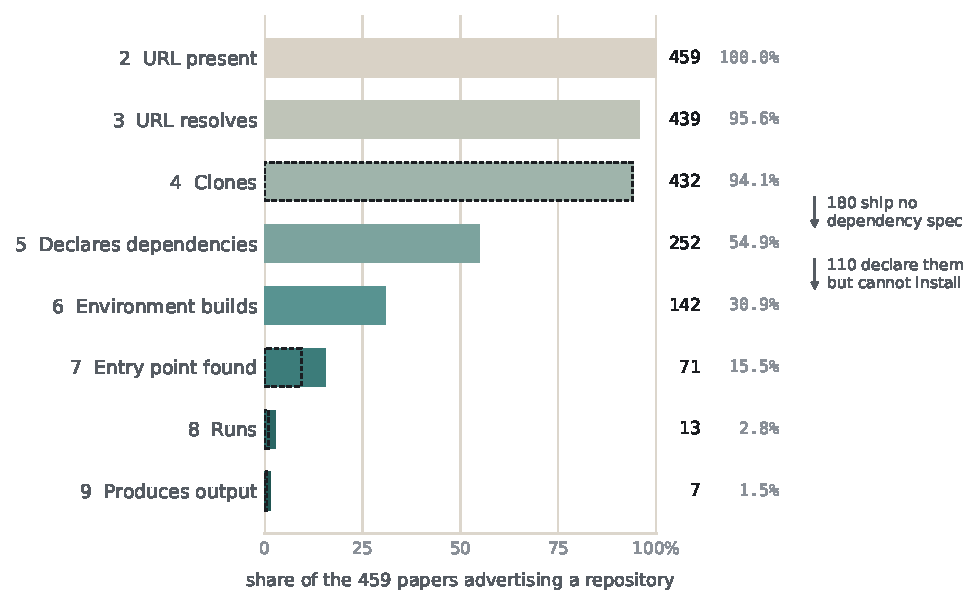
\includegraphics[width=\textwidth]{figures/attrition.pdf}
\caption{The attrition curve, $n=459$ arXiv quantitative-finance
machine-learning papers that advertise a code repository. Filled bars are the
primary specification; dashed outlines show the conservative entry-point rule
where it differs. The two large losses are annotated: they occur at declaring
and building an environment, not at link rot or at execution. Every value is
computed from the released records by \texttt{paper/make\_figures.py}.}
\label{fig:attrition}
\end{figure}

\begin{table}[H]
\centering
\caption{Attrition across the ladder, $n=459$ papers advertising a code URL.
The \emph{README} column is the primary specification, in which entry points may
be taken from the authors' own documentation; the \emph{convention} column
restricts entry points to conventionally named scripts. The two agree exactly
through rung 6, which are decided before any entry-point heuristic applies.}
\label{tab:attrition}
\small
\begin{tabular}{@{}clrrrr@{}}
\toprule
\# & Rung & \multicolumn{2}{c}{README (primary)} & \multicolumn{2}{c}{Convention only} \\
\cmidrule(lr){3-4}\cmidrule(lr){5-6}
   &      & $n$ & \% & $n$ & \% \\
\midrule
2  & \texttt{URL\_PRESENT}       & 459 & 100.0 & 459 & 100.0 \\
3  & \texttt{URL\_RESOLVES}      & 439 & 95.6  & 439 & 95.6 \\
4  & \texttt{CLONED}             & 432 & 94.1  & 431 & 93.9 \\
5  & \texttt{DEPS\_DECLARED}     & 252 & 54.9  & 252 & 54.9 \\
6  & \texttt{ENV\_BUILDS}        & 142 & 30.9  & 142 & 30.9 \\
7  & \texttt{ENTRYPOINT\_FOUND}  & 71  & 15.5  & 43  & 9.4 \\
8  & \texttt{RUNS}               & 13  & 2.8   & 5   & 1.1 \\
9  & \texttt{PRODUCES\_OUTPUT}   & 7   & 1.5   & 3   & 0.7 \\
\bottomrule
\end{tabular}
\end{table}

Three features of the curve carry the paper's content.

\emph{Link rot is real but modest.} Twenty of 459 advertised repositories
(4.4\%) no longer resolve, and one of those twenty is an extraction defect of
ours rather than a dead link, leaving nineteen (4.1\%) as measured rot. This is
the failure mode most often assumed to dominate, and it is the smallest of the
large drops. Two guards stand behind the figure. Because a transient resolver
failure is indistinguishable from a dead domain on a single attempt,
transport-level failures are retried before being recorded; without that, one
repository in this corpus would have been reported as rotted when it was live.
And because an address mangled by text extraction is likewise indistinguishable
from a dead one by status code, the normalization described above is asserted by
the audit script rather than assumed.

\emph{The first large drop is environment declaration.} Of the 432 repositories
that clone, 180 ship no dependency specification of any kind, taking the sample
from 94.1\% to 54.9\% in a single rung. Nothing exotic is required to clear it: a
\texttt{requirements.txt} suffices.

\emph{The second large drop is environment construction.} Of the 252
repositories that declare dependencies, 110 fail to install them, taking the
sample to 30.9\%. \Cref{tab:failure_mix} shows what the installer reported;
\Cref{tab:cohort} shows how the rate varies with the age of the paper. Neither
identifies a mechanism, for reasons given below.

\subsection{Why artifacts stop}\label{sec:failure_mix}

\Cref{fig:reasons} shows every reason an artifact stopped, grouped by the rung
that blocked it; \Cref{tab:failure_mix} gives the same counts as a table. The
single largest bar is not a technical failure at all: 180 repositories ship no
dependency specification, so there is nothing to install.

\begin{figure}[H]
\centering
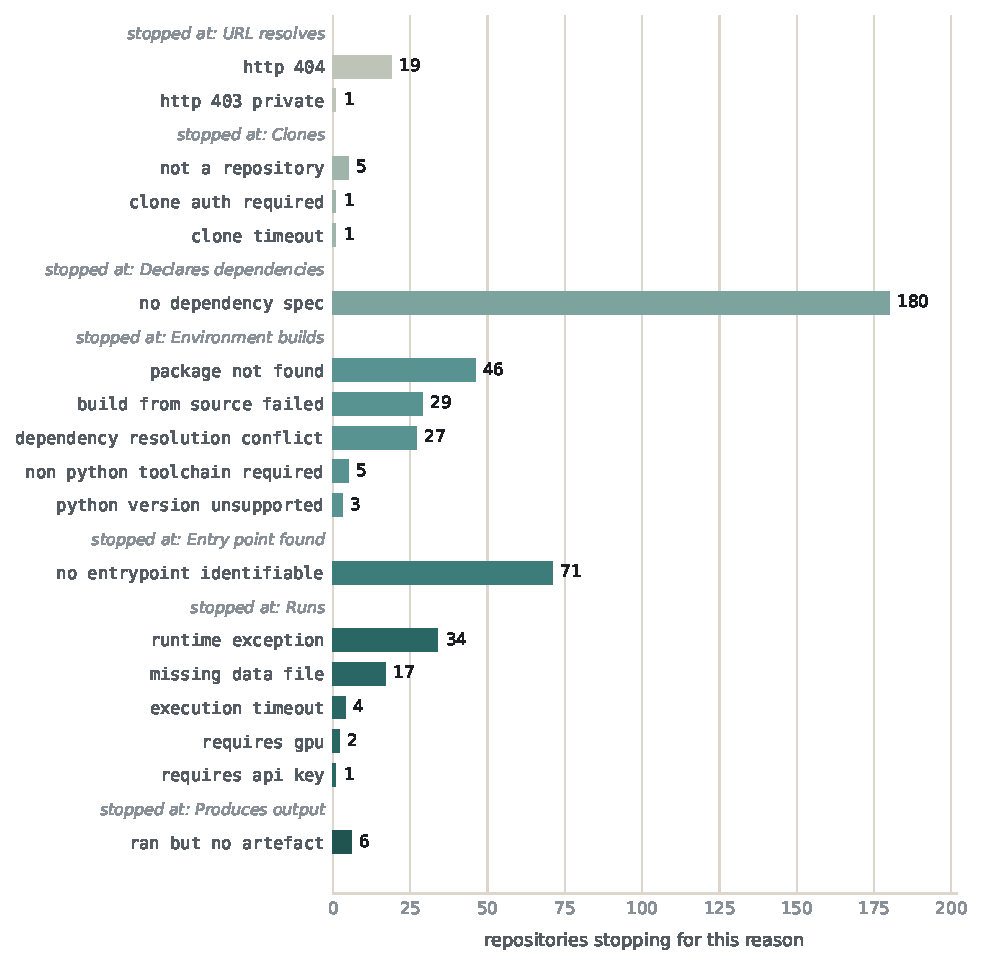
\includegraphics[width=0.92\textwidth]{figures/reasons.pdf}
\caption{Why artifacts stop, primary specification. Each bar counts the
repositories that stopped at the named rung for the named reason; the 452 bars
sum, with the seven artifacts that cleared every mechanical rung, to the full
sample of 459.}
\label{fig:reasons}
\end{figure}

\begin{table}[H]
\centering
\caption{Failure mix by blocking rung, primary specification. Counts are
repositories stopping at that rung for that reason.}
\label{tab:failure_mix}
\small
\begin{tabular}{@{}llr@{}}
\toprule
Rung & Reason & $n$ \\
\midrule
\texttt{URL\_RESOLVES}     & \texttt{http\_404}                       & 19 \\
                           & \texttt{http\_403\_private}              & 1 \\
\midrule
\texttt{CLONED}            & \texttt{not\_a\_repository}              & 5 \\
                           & \texttt{clone\_timeout}                  & 1 \\
                           & \texttt{clone\_auth\_required}           & 1 \\
\midrule
\texttt{DEPS\_DECLARED}    & \texttt{no\_dependency\_spec}            & 180 \\
\midrule
\texttt{ENV\_BUILDS}       & \texttt{package\_not\_found}             & 46 \\
                           & \texttt{dependency\_resolution\_conflict}& 27 \\
                           & \texttt{build\_from\_source\_failed}     & 29 \\
                           & \texttt{non\_python\_toolchain\_required}& 5 \\
                           & \texttt{python\_version\_unsupported}    & 3 \\
\midrule
\texttt{ENTRYPOINT\_FOUND} & \texttt{no\_entrypoint\_identifiable}    & 71 \\
\midrule
\texttt{RUNS}              & \texttt{runtime\_exception}              & 34 \\
                           & \texttt{missing\_data\_file}             & 17 \\
                           & \texttt{execution\_timeout}              & 4 \\
                           & \texttt{requires\_gpu}                   & 2 \\
                           & \texttt{requires\_api\_key}              & 1 \\
\midrule
\texttt{PRODUCES\_OUTPUT}  & \texttt{ran\_but\_no\_artefact}          & 6 \\
\bottomrule
\end{tabular}
\end{table}

The environment failures divide into three roughly comparable mechanisms.
\texttt{package\_not\_found} (46) is a pinned dependency that has left the index;
\texttt{build\_\allowbreak from\_\allowbreak source\_\allowbreak failed} (29) is a
package with no current wheel that fails to compile;
\texttt{dependency\_\allowbreak resolution\_\allowbreak conflict} (27) is the
residual, and it is a weaker label than its name suggests. It is the classifier's
fallthrough, so it collects genuine pin conflicts together with build-backend
errors that resist finer classification. We report it as a bucket rather than a
mechanism, and a reader wanting the split can recover it from the stored
installer output in the released records. All three are properties of elapsed
time rather than of the authors' diligence at submission. Whether that amounts to
decay is a question the corpus can be asked directly, and the answer is more
qualified than we first assumed.

\begin{table}[H]
\centering
\caption{Environment construction by publication cohort, primary specification.
Cohort is the year in the arXiv identifier's \texttt{YYMM} prefix, that is the
month the paper was announced and the artifact became publicly reachable, which
is the clock an aging artifact runs on. Three of the 459 records were submitted
in the calendar year before their identifier was issued and would fall one
cohort earlier under the corpus \texttt{year} field; two of those sit on the
2025/2026 boundary and move 137/68 to 139/66. The rightmost column, and every
claim drawn from it, is identical under either rule. That column conditions on
the repository having declared dependencies at all, so it isolates whether a
declared environment can still be built.}
\label{tab:cohort}
\small
\begin{tabular}{@{}lrrrr@{}}
\toprule
Cohort & $n$ & Declares deps & Builds & Builds $\mid$ declares \\
\midrule
2015--2022 & 64  & 45.3\% & 18.8\% & 41.4\% \\
2023       & 68  & 54.4\% & 22.1\% & 40.5\% \\
2024       & 122 & 49.2\% & 27.0\% & 55.0\% \\
2025       & 137 & 61.3\% & 38.7\% & 63.1\% \\
2026       & 68  & 61.8\% & 42.6\% & 69.0\% \\
\bottomrule
\end{tabular}
\end{table}

The gradient is real but modest, and it is not monotone: conditional on declaring
dependencies, a 2026 artifact builds about 1.7 times as often as one from 2022 or
earlier, and the 2023 cohort sits marginally below the oldest one. An earlier
version of this table showed a threefold gradient; roughly half of it was a
defect in our own container image, which penalized exactly the older repositories
most likely to need a source build (\Cref{sec:harness_defects}). We report the
corrected figures and note that our first, more striking result was wrong in the
direction we would have liked.

Two readings fit what remains, and a single cross-section cannot separate them.
Artifacts may decay as they age, or practice may simply be improving, so that
recent authors write more buildable environments than their predecessors did.
Both are plausible, and at this effect size neither is strongly supported.

The reason mix argues against attributing the gradient wholly to the mechanism we
had assumed. If aging worked mainly through packages leaving the index, then
\texttt{package\_not\_found} should claim a growing share of older cohorts. It
does not: as a fraction of repositories that declare dependencies it is 17.2\%
for 2015--2022, 29.7\% for 2023, 16.7\% for 2024, 16.7\% for 2025 and 14.3\% for
2026, which is flat within sampling noise. The honest statement is that older
artifacts build less often, that the mechanism is not identified by these data,
and that separating decay from cohort requires re-scoring this corpus later
rather than reasoning across it now. The harness is released so that measurement
can be made.

This also means the measurement is timestamped: the same corpus scored two years
hence is unlikely to score the same, and any comparison against these figures
must carry their date.

At the execution rung, the seventeen \texttt{missing\_data\_file} outcomes are
substantive, though the label is broader than its name. The classifier routes any
report of an absent path to this bucket, which covers two situations: a
repository that fetches its inputs at run time and is blocked because network
access is denied during execution by design, and a repository whose expected
input file simply is not in the distribution. Both mean the same thing for a
reader, which is why they share a rung, and neither is rescued by our
connectivity: the artifact as released does not carry what it needs. They are not
separated in the counts, and a reader wanting the split can recover it from the
per-record detail in the released data, which is now retained at full length for
this purpose.

\subsection{Defects found in our own instrument}\label{sec:harness_defects}

A study that measures how often other people's code silently fails is obliged to
report how often its own did. Four defects were found after a first campaign had
completed, and they did not all err in the same direction. Three inflated the
failure rate, in the direction this study's hypothesis predicted, which is why
they were hard to see: a harness that agrees with you invites less scrutiny. The
fourth did the opposite and manufactured a success, which is the error a reader
should worry about more, and it was caught only because the output was read
rather than counted.

\emph{The container image lacked a toolchain.} The base image was
\texttt{python:3.11-slim}, which ships neither \texttt{git} nor a C compiler. A
repository whose requirements name a \texttt{git+https} dependency, or whose
wheel must be compiled, therefore failed to install for a reason belonging to our
image. Seven repositories were affected, four for want of \texttt{git} and three
for want of a compiler.

\emph{The clone was shallow.} \texttt{git clone -{}-depth 1} fetches no tags, and a
package whose version is derived by \texttt{setuptools-scm} then fails with
``unable to detect version''. Eight repositories failed to build for that reason
alone. A reader following the paper's URL clones normally and sees none of this.

\emph{A bare \texttt{make} was accepted as an entry point.} The documented rule
has always been that a command taken from a README must name a target that
exists; the code checked only that a \texttt{Makefile} was present. One
repository's default target printed the Makefile's own usage message, and an
interim run recorded that as the artifact producing output at rung 9. This is the
defect that ran the wrong way: it created a success rather than a failure, and it
would have added an eighth paper to the headline count. It is the second such
case in this project's history, the first being a vendored tokenization library
whose bundled demo satisfied the naming heuristic for two papers
(\Cref{sec:ladder}); both are visible in the superseded result files released
alongside the current ones.

\emph{URL normalization stripped only trailing characters}, as described in
\Cref{sec:corpus}.

The first three matter for the shape of the curve, not merely its level. Older
repositories are the ones most likely to need a source build or a \texttt{git}
dependency, so the missing toolchain penalized them disproportionately.
Conditional on declaring dependencies, the 2015--2022 cohort builds 41.4\% of the
time under the corrected harness and 20.7\% under the defective one, while the
2026 cohort is unchanged at 69.0\%. Roughly half of what had looked like an age
gradient was our own image. The remaining gradient is reported in
\Cref{tab:cohort} and is considerably milder.

We report this at length because the alternative was to report a cleaner result
that we knew to be partly an artifact, and because the pattern is the paper's own
argument turned on itself: the defects were invisible precisely because their
output was plausible.

\subsection{Not every advertised repository is the paper's own}\label{sec:shared_repos}

The 459 records point to 427 distinct repositories. Twenty-five addresses are
advertised by more than one paper, accounting for 57 records, and inspection of
that list shows what is happening: several are widely used third-party libraries
rather than a paper's released code. A paper that names the data client or the
modeling toolkit it used, in the same sentence pattern a paper uses to announce
its own repository, is indistinguishable to an extractor working from prose.

These records behave differently enough to matter. Repositories shared between
papers clone 100.0\% of the time against 93.3\% for the rest, declare
dependencies 86.0\% against 50.5\%, and build 50.9\% against 28.1\%. That is what
a maintained library looks like. But they yield an entry point 14.0\% of the time
against 15.7\%, and \emph{none} of them produces output, because a library has no
analysis to run. Including them therefore lifts the middle of the curve
while contributing nothing at the top, which flatters the environment rungs and
makes the drop from rung 6 to rung 9 look steeper than it is for the papers'
own artifacts.

We report the unscreened curve as primary because the screening rule we can
implement is a heuristic in its own right, and substituting one heuristic for
another silently would be worse than disclosing this one. A reader who wants the
screened figure can recompute it from the released records, and the direction of
the bias is stated here so that no one has to guess at it. The effect on the
paper's conclusion is small and adverse to our own headline: excluding shared
repositories would lower the environment rungs and leave the seven rung-9
artifacts untouched.

\subsection{Sensitivity to the entry-point heuristic}\label{sec:sensitivity}

Identifying what to run is the most discretionary step, so the study is run in two
configurations. Restricting to conventionally named scripts finds an entry point
in 43 repositories; additionally accepting a command documented in the
repository's own README finds 71. The looser specification raises the number that
execute from 5 to 13 and the number that emit output from 3 to 7.

The sensitivity carries through to the top of the ladder, and it must be reported
there because that is where it bites hardest. The single artifact scored
\emph{match} at rung 10 is reached only by the README route: under the
conservative rule it never clears rung 7. Of the three artifacts that do emit
output under that rule, two are the bundled self-tests of
\Cref{sec:rung10_results}. The third is the timing case described above: a
completed portfolio backtest, which is a more substantial run than anything in
the primary rung-9 set apart from the match itself. It was adjudicated
separately and scored \emph{not comparable}, on two grounds: the paper's abstract
states no recoverable numeric claim, reporting only that the method
``significantly outperforms'' its baselines, and the run seeds itself randomly
and says so in its own output, so a second run would emit different values. The
adjudicated match count is therefore one under the primary specification and zero
under the conservative one, with all eight adjudications released in the
worksheet. The adjudicated match count is therefore one under the
primary specification and zero under the conservative one. Stopping the sensitivity analysis at rung 9, where the two columns still
show a difference of degree, would have concealed the one place where the
headline changes in kind.

The two configurations agree on rungs 2 through 6 for 458 of the 459
repositories, and the audit script checks that they agree to within that
tolerance. Both exceptions we have observed are wall-clock effects rather than
scoring disagreements, and both are worth stating because they bound how
reproducible these figures are.

One repository cloned in one run and hit the ten-minute clone timeout in the
other. Unlike the resolution check at rung 3, the clone is not retried, so a slow
transfer is recorded as a failure. A second repository, with the same
conventionally named entry point selected in both runs, completed in 1{,}667
seconds under one configuration and exceeded the 1{,}800-second execution budget
under the other. It is therefore the one record whose conservative rung
\emph{exceeds} its primary rung, so the conservative set is not a subset of the
primary at rungs 8 and 9 even though the entry-point rule is strictly stricter.
Three artifacts emit output under the conservative rule and seven under the
primary, but the two sets are not nested: one member of the smaller set is absent
from the larger.

The practical reading is that the mechanical rungs are reproducible to within
about one repository, that the upper rungs additionally carry timing sensitivity
for artifacts whose runtime sits near the budget, and that a headline of seven is
seven plus or minus one rather than an exact count.

The gap between the columns is the honest measure of how much of the upper curve
is our conservatism rather than the literature's. It is large in relative terms
and small in absolute terms: on either specification, fewer than one paper in
thirty executes to completion unassisted, and fewer than one in sixty emits
output.

\subsection{Comparison with the earlier, smaller campaign}\label{sec:replication}

An earlier campaign scored a 154-paper sample. Those 154 papers are a strict
subset of the present 459: the corpus was extended rather than redrawn, so every
paper in the earlier campaign is also in this one. We state that plainly because
comparing the subset against the superset that contains it would not be a
replication, and reporting it as one would be the most misleading thing in this
paper.

Nor can the two campaigns be compared as repeated measurements. The harness
changed between them, and not cosmetically: the container image gained a
toolchain, the clone stopped being shallow, and the entry-point rule was
tightened (\Cref{sec:harness_defects}). Five of the 154 records differ across the
campaigns at rungs 2 to 6, and all five are consequences of those revisions. The
comparison therefore measures our corrections, not the literature, and we draw no
stability conclusion from it.

What can be compared out of sample is the 305 papers that entered with the
expansion and that the earlier campaign never saw, scored under the same harness
as everything else. Restricting to rungs 2 through 6, the earlier 154 score
resolution 94.2\%, cloning 89.6\%, dependency declaration 53.9\% and environment
construction 27.9\%; the 305 added papers score 96.4\%, 96.4\%, 55.4\% and
32.5\%. Declaration differs by 1.5 percentage points and construction by 4.5.

Those crude gaps should not be read as stability, and the reason is worth setting
out because it is easy to miss. The two partitions have very different age
profiles: the earlier 154 contain no paper announced before 2024, while the added
305 reach back to 2015 and are 21\% pre-2023. Within every cohort the two
partitions share, the added papers build far more often than the earlier ones:
29.0\% against 13.3\% for 2024, 62.5\% against 25.8\% for 2025, and 61.1\%
against 36.0\% for 2026. Standardizing the added partition's cohort-specific
rates onto the earlier partition's age mix gives 58.8\% against 27.9\%, a gap of
thirty points rather than four and a half.

The near-agreement in the crude figures is therefore composition canceling
outcome: the added sample is older, which lowers its overall rate, and better
within each cohort, which raises it. We do not know why the two partitions differ
so much within cohort. It is not the seed set carried over from earlier work
(excluding it leaves the earlier partition at 28.4\%), and it is not where the
URL was found (papers whose URL came from the abstract and from the full text
build 26.5\% and 32.1\% of the time respectively, a gap far smaller than the one
to be explained). The honest reading is that the two draws
are not exchangeable, that we cannot say what distinguishes them, and that this
study therefore has no strong out-of-sample check. The shape of the curve, two
large losses at declaration and construction, is common to both partitions; the
levels are not.

\subsection{Rung 10}\label{sec:rung10_results}

Seven repositories produced output and are therefore eligible for the final rung,
which asks whether an emitted number matches a headline number in the paper. All
seven were adjudicated by hand against the paper's own numeric claims; the
worksheet pairing each artifact's captured stdout with those claims is released
with the corpus so the judgments can be inspected and disputed. One was scored
\emph{match} and six \emph{not comparable}. We give the count rather than a rate:
seven cannot support a percentage.

Reading the seven is more informative than counting them, because it shows that
rung 9 is a weaker rung than its name suggests. Emitting output is not the same
as running the analysis. Two artifacts executed a bundled self-test that reports
tensor shapes and losses on synthetic inputs. One ran a correctness validator
that skipped every GPU check because the CUDA extensions were not built, which
is precisely where the paper's throughput claims come from. One completed a
walk-forward experiment whose data fetch returned nothing for every ticker, so
the analysis ran on an empty universe. One terminated on a missing API key, and
the captured output is that error. One ran a data-acquisition step that wrote
files and printed nothing.

The single \emph{match} is instructive about what success looks like, and it was
checked against the published table rather than taken on the script's word. The
repository documents \texttt{finalscripts/table1.py}; running it regenerates the
paper's Table 1 in full, on the same 14-variable panel, and every one of the
thirty-six reported values agrees exactly: recall, precision, $F_1$ and mean
signed offset for all nine methods, from \texttt{LLM only} at
$0.77/0.87/0.82/{+}3.1$ through the four data-only baselines to the four
cross-validated variants, ending at $0.88/0.77/0.82/{+}0.9$. The best $F_1$ of
0.82 is the figure the abstract headlines. Presentation differs without
disagreeing: the manuscript labels the combined rows differently from the script,
reports an $F_2$ column the script omits, and omits the raw hit and false-alarm
counts the script prints.

What reproduced, however, is narrower than ``regenerates Table 1'' suggests, and
the artifact says so itself. Its output header reports \texttt{new API calls =
0}: the language-model stage over central-bank minutes, which is the paper's
distinctive contribution, is replayed from model outputs committed to the
repository rather than recomputed. Network access is denied during execution, so
it could not have been otherwise. What runs end to end is the statistical
validation and scoring on stored text-derived candidates, which is a real and
unusually well-packaged result, but it is not the text pipeline. We record this
because a paper arguing that ``reproduced'' is used too loosely cannot afford to
use it loosely about its own single success.

One artifact in 459 regenerated a published table on a clean machine, from the
URL the paper gives its readers, without network access and without contacting
anyone, on model outputs the authors had the foresight to commit.

That the sample thins from 459 to seven, and from seven to one, is itself the
finding: the question the rung was designed to answer is, for this corpus, very
nearly unanswerable, because almost nothing gets far enough to ask it of.
